\documentclass[10pt]{article}
% for pdflatex
\usepackage[utf8]{inputenc}
% for hyperlink
\usepackage{hyperref}
\hypersetup{
    colorlinks=true,
    linkcolor=blue,
    filecolor=magenta,
    urlcolor=cyan,
}
% for custom enum
\usepackage{enumitem}
% for removing alinea begin of paragraph
\usepackage{parskip}
\usepackage{array, xcolor, graphicx}
\usepackage[a4paper, margin=1cm]{geometry}

% path of figures and pictures
\graphicspath{{figures/}}

\title{\bfseries\Huge Ingénieur Blockchain \& DevOps \vspace{-4ex}}
% no author
\author{\bfseries\Huge \vspace{-4ex}}
% no date
\date{}
% custom for column style
\definecolor{lightgray}{gray}{0.8}
% custom for column type
\newcolumntype{L}{p{0.18\textwidth}}
% custom for column type
\newcolumntype{R}{p{0.75\textwidth}}
% custom for column type
\newcommand\VRule{\color{lightgray}\vrule width 2pt}
% for bullet point outside of list
\newcommand{\tabitem}{~~\llap{$\rightarrow$}~~}
\begin{document}

\begin{minipage}[t]{0.80\textwidth}
\textbf{Mohamed Amine LEGHERABA}\\
25 ans\\
92 bis rue Rouget de Lisle, Bezons, France\\
\href{tel:0630829000}{06 30 82 90 00}\\
\href{mailto:mlegheraba@protonmail.com}{mlegheraba@protonmail.com}\\
\href{https://github.com/MohamedLEGH}{github.com/MohamedLEGH} \\

{\bf Français}: langue maternelle \\
{\bf Anglais}: bon niveau (TOIEC: 935) \\
\end{minipage}
\begin{minipage}[t]{0.20\textwidth}
\vspace{-3ex}
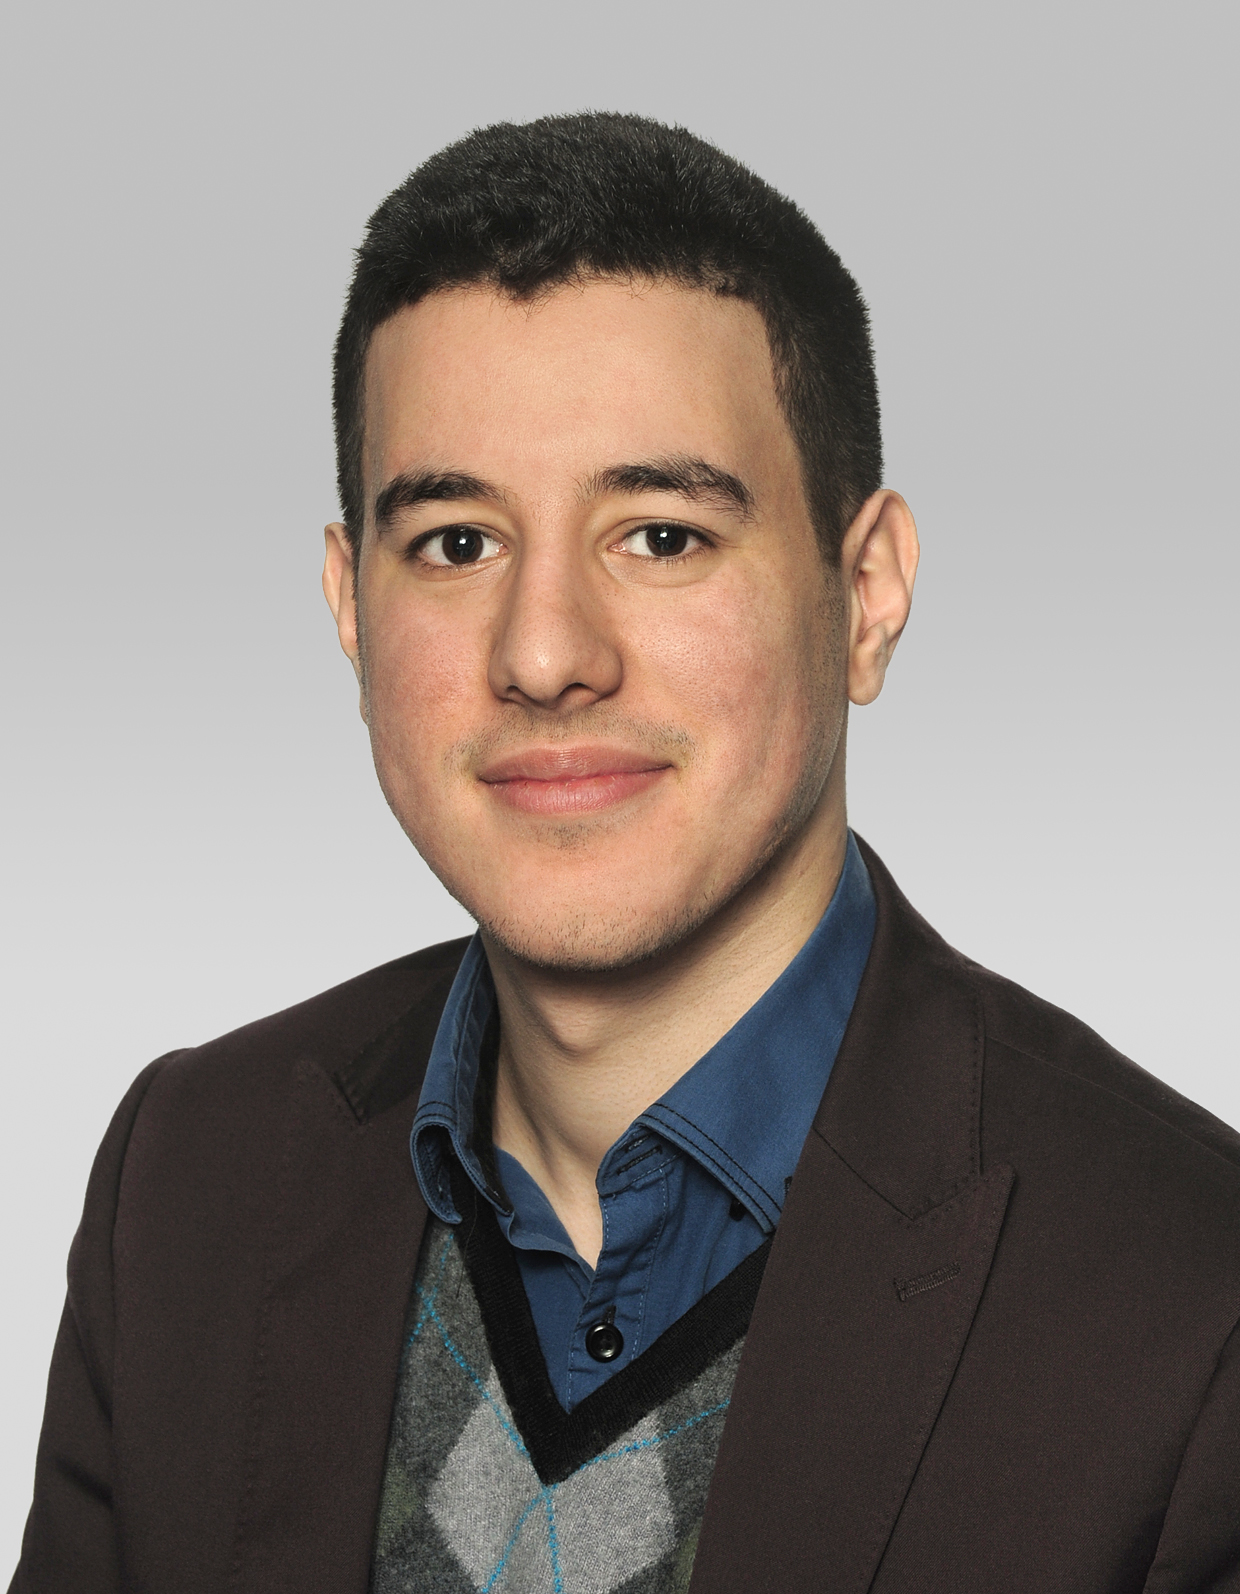
\includegraphics[width=3cm]{Legheraba-Mohamed.jpg}
\end{minipage}
\vspace{-8ex}
% to make maketitle work without begin of page
{\let\newpage\relax\maketitle}
% to remove page number
\thispagestyle{empty}

\vspace{-8ex}

\section*{Formation}
\begin{tabular}{L!{\VRule}R}
\textbf{\textit{2015--2018}} & \textbf{École d'ingénieurs Polytech Sorbonne}, spécialité \textit{Mathématiques Appliquées et Informatique Numérique}. Semestre Erasmus aux Pays-Bas (TU Delft) en Hiver 2017.\\[0.75cm]
\textbf{\textit{2013--2015}} & \textbf{École d'ingénieurs Polytech Sorbonne}, classe \textit{PeiP} (Préparation aux écoles d'ingénieurs Polytech)\\[0.75cm]
\textbf{\textit{2013}}&\textbf{Baccalauréat S}, mention Bien. Lycée Chaptal. \\
\end{tabular}


\section*{Expérience Professionnelle}
\begin{tabular}{L!{\VRule}R}
\textbf{\textit{Depuis 2019}}& 
\includegraphics[width=2cm]{SIA_logo.png} \hspace{0.2cm} {\bf Ingénieur Blockchain \& DevOps, Sia Partners} \\[0.25cm]

& \tabitem \small{\textbf{Développement d'applications blockchain pour les clients de Sia Partners} (réseau Corda pour un gestionnaire d'actifs, application mobile de paiement en cryptomonnaie, ...)}

\\[0.20cm]
& \tabitem \small{\textbf{Projet Heka: \href{https://heka.sia-partners.com/fr}{Usine logicielle} pour les applications Data Science} (développement des microservices en Python et en React, déploiement continu sur l'infrastructure Kubernetes, ...)}

\\[0.20cm]
& \tabitem \small{\textbf{Veille R\&D sur la blockchain et les cryptomonnaies} (étude des réseaux blockchain Liquid, Libra et TON, des technologies Lightning Network, Taproot et Multi-Party Computation, ...)}

\\[0.20cm]
& \tabitem \small{\textbf{Rédaction d'articles} (\href{https://www.sia-partners.com/fr/actualites-et-publications/de-nos-experts/la-blockchain-catalyseur-de-la-decentralisation-et-de-la}{\textit{Blockchain \& 5G}}, \href{https://www.sia-partners.com/fr/actualites-et-publications/de-nos-experts/entretien-avec-pierre-noizat-bitcoin-et-cryptomonnaies-0}{\textit{Interview de Pierre Noizat}}, ...)}

\\[0.20cm]
& \tabitem \small{\textbf{Enseignement \textit{Programmer une blockchain}} (\href{https://github.com/MohamedLEGH/tutoriel-blockchain-creation-bootstrap}{Polytech Sorbonne}, \href{https://github.com/MohamedLEGH/tutoriel-blockchain-MinesBootstrap}{Mines St Etienne}, ...)}

\\[0.20cm]
\textbf{\textit{Mars--Septembre 2018}}& 
\includegraphics[width=1.5cm]{ofi-am.png} \hspace{0.2cm} {\bf Stagiaire veille R\&D, Département Développement, OFI AM, 6 mois}.\\
& \small{Veille autour des technologies de Blockchain, de l’automatisation de tâches avec Airflow, de la conteneurisation d’application avec Docker et de la supervision système avec Tableau Server.} \\

\end{tabular}


\section*{Compétences}
\begin{tabular}{ l l }
\textbf{Blockchain}: Bitcoin, Ethereum, Hyperledger, Corda & \textbf{DevOps}: Kubernetes, Gitlab CI/CD, GCP, Terraform \\[0.1cm]
\textbf{Smart contracts}: Solidity, Bitcoin Script, Chaincodes & \textbf{Outils}: Shell, Git, Docker, VS Code, PowerPoint \\[0.1cm]
\textbf{Mathématiques}: Cryptographie, Statistiques, Graphes & \textbf{Programmation}: Python, JavaScript, C/C++, Bash  \\[0.1cm]
\textbf{Bases de données}: MySQL, PostgreSQL, SQLAlchemy & \textbf{Frameworks}: ReactJS, Node.js, Flask, PyQt, R Shiny \\[0.1cm]
\textbf{Protocoles}: Lightning Network, IPFS, BitTorrent & \textbf{Méthodologie}: Méthode Agile, APIs REST, Microservices \\[0.1cm]
\end{tabular}

\section*{Contributions Associatives}
\begin{tabular}{L!{\VRule}R}
\textbf{\textit{Depuis 2018}} & Association \textbf{Le Trait D’Union}, Aide aux devoirs auprès de lycéens et de collégiens. Rédaction de dossiers de subventions. \\[0.75cm]

\textbf{\textit{2014--2017}} & Association étudiante \textbf{Averroès}, Dons alimentaire pour les étudiants, trésorier puis président. \\
\end{tabular}
\section*{Loisirs}
\hspace*{1ex} \textbf{Électronique} (console retrogaming avec un Raspberry Pi, contrôle d'un ventilateur via un transistor, ...) \\
\hspace*{1ex} \textbf{Étude des doctrines socio-économiques} (libéralisme, école autrichienne d'économie, anarchisme, technoéthique, ...) \\
\end{document}
